\documentclass[tikz,border=6pt]{standalone}
\usepackage[T1]{fontenc}
\usepackage[utf8]{inputenc}
\usepackage{pgfplots}
\usepgfplotslibrary{groupplots}
\usetikzlibrary{calc}
\pgfplotsset{compat=1.18}
\begin{document}
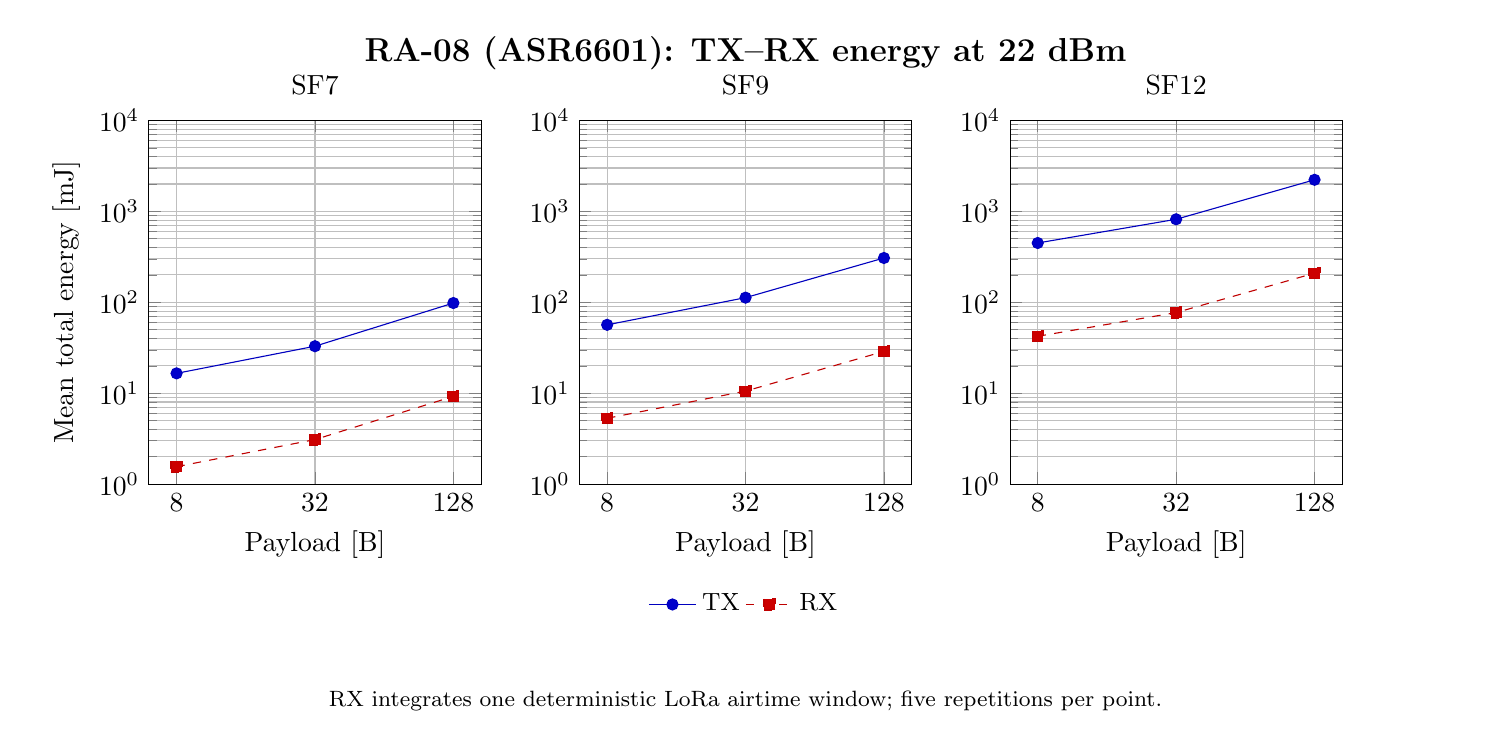
\begin{tikzpicture}
\begin{groupplot}[/pgf/number format/use comma, group style={group size=3 by 1, horizontal sep=1.25cm},
  width=5.8cm,height=6.2cm,xmode=log,log basis x=2,ymode=log,log basis y=10,ymin=1,ymax=10000,
  xtick={8,32,128},xticklabels={8,32,128},grid=both,xlabel={Payload [B]},
  legend style={draw=none,fill=none,font=\small,at={(0.5,-0.27)},anchor=north,legend columns=-1}]
% TX--RX energy
\nextgroupplot[title={SF7},ylabel={Mean total energy [mJ]}]
\addplot+[blue!75!black,solid,mark=*,error bars/.cd,y dir=both,y explicit] coordinates {(8,16.5149661) +- (0,0.0215876065) (32,32.8358955) +- (0,0.0946227038) (128,98.0504253) +- (0,0.257586409)};
\addplot+[red!75!black,dashed,mark=square*,error bars/.cd,y dir=both,y explicit] coordinates {(8,1.55393958) +- (0,0.00392974637) (32,3.08659502) +- (0,0.00739410574) (128,9.21915455) +- (0,0.012521578)};
\nextgroupplot[title={SF9}]
\addplot+[blue!75!black,solid,mark=*,error bars/.cd,y dir=both,y explicit] coordinates {(8,56.4390596) +- (0,0.124893974) (32,112.374425) +- (0,0.23018278) (128,306.862201) +- (0,0.400943568)};
\addlegendentry{TX}
\addplot+[red!75!black,dashed,mark=square*,error bars/.cd,y dir=both,y explicit] coordinates {(8,5.29276633) +- (0,0.00719189946) (32,10.5388417) +- (0,0.00868118935) (128,28.8005093) +- (0,0.0526185386)};
\addlegendentry{RX}
\nextgroupplot[title={SF12}]
\addplot+[blue!75!black,solid,mark=*,error bars/.cd,y dir=both,y explicit] coordinates {(8,448.614794) +- (0,0.656256626) (32,817.933317) +- (0,0.808675368) (128,2223.05304) +- (0,0.965374333)};
\addplot+[red!75!black,dashed,mark=square*,error bars/.cd,y dir=both,y explicit] coordinates {(8,42.2235158) +- (0,0.0165906389) (32,77.0234732) +- (0,0.104623399) (128,208.885987) +- (0,0.0857955427)};
\end{groupplot}
\node[font=\bfseries\large] at ($(group c2r1.north)+(0,0.85cm)$) {RA-08 (ASR6601): TX--RX energy at 22 dBm};
\node[font=\footnotesize,align=center,text width=18cm] at ($(group c2r1.south)+(0,-2.75cm)$) {RX integrates one deterministic LoRa airtime window; five repetitions per point.};
\end{tikzpicture}
\end{document}
